\documentclass[11pt]{article}

\usepackage{centernot}
\usepackage{amssymb}
\usepackage{xcolor}
\definecolor{myblue}{RGB}{0, 0, 255} 
\definecolor{mygreen}{RGB}{0, 180, 80}
\definecolor{myred}{RGB}{153, 0, 0}
\definecolor{myorange}{RGB}{255, 153, 51}
\definecolor{mypurple}{RGB}{102, 0, 204}
\usepackage{verbatim}
\usepackage{multicol}
\usepackage{enumitem}
\usepackage{amsfonts}
\usepackage{amsmath}
\usepackage[utf8]{inputenc}
\usepackage[export]{adjustbox}  % for correct logo rendering
\usepackage{fancyhdr}  % for header/footer formatting
\usepackage{hyperref}  % for hyper-references
\usepackage{datetime}  % to update month in footer
\usepackage{array}  % more flexible tables
\usepackage[includeheadfoot,
            left=1in,
            right=1in,
            top=0.75in,
            bottom=0.75in,
            headheight=40pt]{geometry} % geometry needs to know headheight to correctly render the footer
\usepackage{tikz} % For drawing grid boxes

\definecolor{darkblue}{RGB}{0, 0, 139}
\definecolor{lightblue}{RGB}{173, 216, 230}

% desired format for footer
\newdateformat{monthyeardate}{%
  \monthname[\THEMONTH] \THEYEAR}

% set up header/footer
\pagestyle{fancy}
\fancyhf{}  % clear all headers/footers
\renewcommand{\headrulewidth}{0pt}  % remove header rule
\renewcommand{\footrulewidth}{0pt}  % remove footer rule

% set up header

\fancypagestyle{firstpage}{
    \fancyhead[L]{
    \vspace{0pt}
    \hspace{-8pt}
    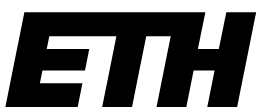
\includegraphics[width=0.1\textwidth]{docimgs/eth_logo_kurz_pos.png}\\
    \textbf{Swiss Federal Institute of Technology}\\
    \textbf{Zurich}\\
    %\textbf{ } \\
    
    }    

    \fancyhead[R]{
    \raggedleft
    %\vspace{20pt}
    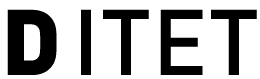
\includegraphics[width=0.13\textwidth]{docimgs/eth_ditet_logo_pos.png}\\
     \textbf{Dept. of Information Technology and} \\ \textbf{Electrical Engineering}  \\
     %\textbf{Chair for Mathematical Information} \\ \textbf{Information Science} \\

    }
}

% set up footer
\fancyfoot[L]{mdietz, ÜS 12}
\fancyfoot[C]{\thepage}
\fancyfoot[R]{\monthyeardate\today}

% set up section/subsection titles
\renewcommand{\thesection}{\arabic{section}}
\renewcommand{\thesubsection}{\arabic{subsection}}

% command used for simply emphasizing suggestions
\newcommand{\suggestion}[1]{{\itshape #1}}

%--- commands for transform arrows----------------
\newcommand{\transform}[2]{%
    \begin{tikzpicture}
        % Open circle
        \draw[thick] (0,0) circle (0.1);
        % Line with number above and adjustable length
        \draw[thick] (0.1,0) -- (#2,0) node[midway, above] {#1};
        % Filled circle
        \filldraw[thick] (#2,0) circle (0.1);
    \end{tikzpicture}%
}
\newcommand{\invtransform}[2]{%
    \begin{tikzpicture}
        % filled circle
        \filldraw[thick] (0,0) circle (0.1);
        % Line with number above and adjustable length
        \draw[thick] (0.1,0) -- (#2 -0.1,0) node[midway, above] {#1};
        % open circle
        \draw[thick] (#2,0) circle (0.1);
    \end{tikzpicture}%
}
\newcommand{\verticaltransform}[4]{%
    \begin{tikzpicture}
        % Open circle at the bottom with text below
        \filldraw[thick] (0,0) circle (0.1) node[below=3pt] {$#4$};
        % Vertical line with number on the left
        \draw[thick] (0,0.1) -- (0,#2 -0.1) node[midway, left] {#1};
        % Filled circle at the top with text above
        \draw[thick] (0,#2) circle (0.1) node[above=3pt] {$#3$};
    \end{tikzpicture}%
}
\newcommand{\verticalinvtransform}[4]{%
    \begin{tikzpicture}
        % Open circle at the bottom with text below
        \draw[thick] (0,0) circle (0.1) node[below=3pt] {$#4$};
        % Vertical line with number on the left
        \draw[thick] (0,0.1) -- (0,#2) node[midway, left] {#1};
        % Filled circle at the top with text above
        \filldraw[thick] (0,#2) circle (0.1) node[above=3pt] {$#3$};
    \end{tikzpicture}%
}

\begin{document}
\thispagestyle{firstpage}

\setlength{\headheight}{1 \baselineskip}  % accomodate header
\setlength{\parindent}{0pt}  % remove initial paragraph indent
\setlength{\parskip}{\baselineskip}  % add skip between paragraphs

\vspace*{-5px}
\section*{Übungsstunde 12}

\section*{Themenüberblick}
\begin{itemize}
    \item \textbf{Diskrete Fouriertransformation (DFT)}
    \item[] Kurze Repetition
    \item[] Diskrete Filter, Überabtastung, Unterabtastung
    \item \textbf{Fast Fourier Transform (FFT)}
    \item[] Cooley-Tukey FFT
    \item \textbf{Tipps für die Prüfung}
\end{itemize}

\section*{Aufgaben für diese Woche}
\vspace{-0.5cm}

\textbf{123}, \textbf{124}, \textbf{125}, \textbf{126}, \textbf{127}, \textbf{128}, \textbf{129}, \textbf{130}, \textbf{131}\\
\vspace{-0.5cm}

Die meisten Übungen überschneiden sich mit letzter Woche.

Die \textbf{fettgedruckten} Übungen empfehle ich, weil sie wesentlich zu eurem Verständnis der Theorie beitragen und/oder sehr prüfungsrelevant sind.

Die DFT ist \textcolor{myred}{sehr wichtig}! Es kommt immer eine ganze Aufgabe dazu an der Prüfung. (25 / 100P)

\vfill \null
\pagebreak

\section*{Diskrete Fouriertransformation (DFT)}
\vspace*{-0.5cm}

\fcolorbox{darkblue}{lightblue}{%
    \parbox{\dimexpr\linewidth-2\fboxsep-2\fboxrule\relax}{
    \vspace*{0.15cm}
    \begin{itemize}
        \item[] $(\textbf{DFT}) \hspace{80pt} \hat{x}[k] = \displaystyle\sum_{n=0}^{N-1} x[n]\omega_N^{kn} \hspace{80pt} \hat{x}[k+N] = \hat{x}[k]$
        \item[] $(\textbf{IDFT}) \hspace{76pt} x[n]=\displaystyle\frac{1}{N}\displaystyle\sum_{k=0}^{N-1} \hat{x}[k] \omega_N^{-kn} \hspace{58pt} x[n+N] = x[n]$
        \item[] wobei $\hspace{88pt} \omega_N = e^{-\frac{2 \pi i}{N}}$
    \end{itemize}
}}%

\subsection*{Visualisierung der verschiedenen Fouriertransformationen}
\vspace*{-0.5cm}
\begin{center}
    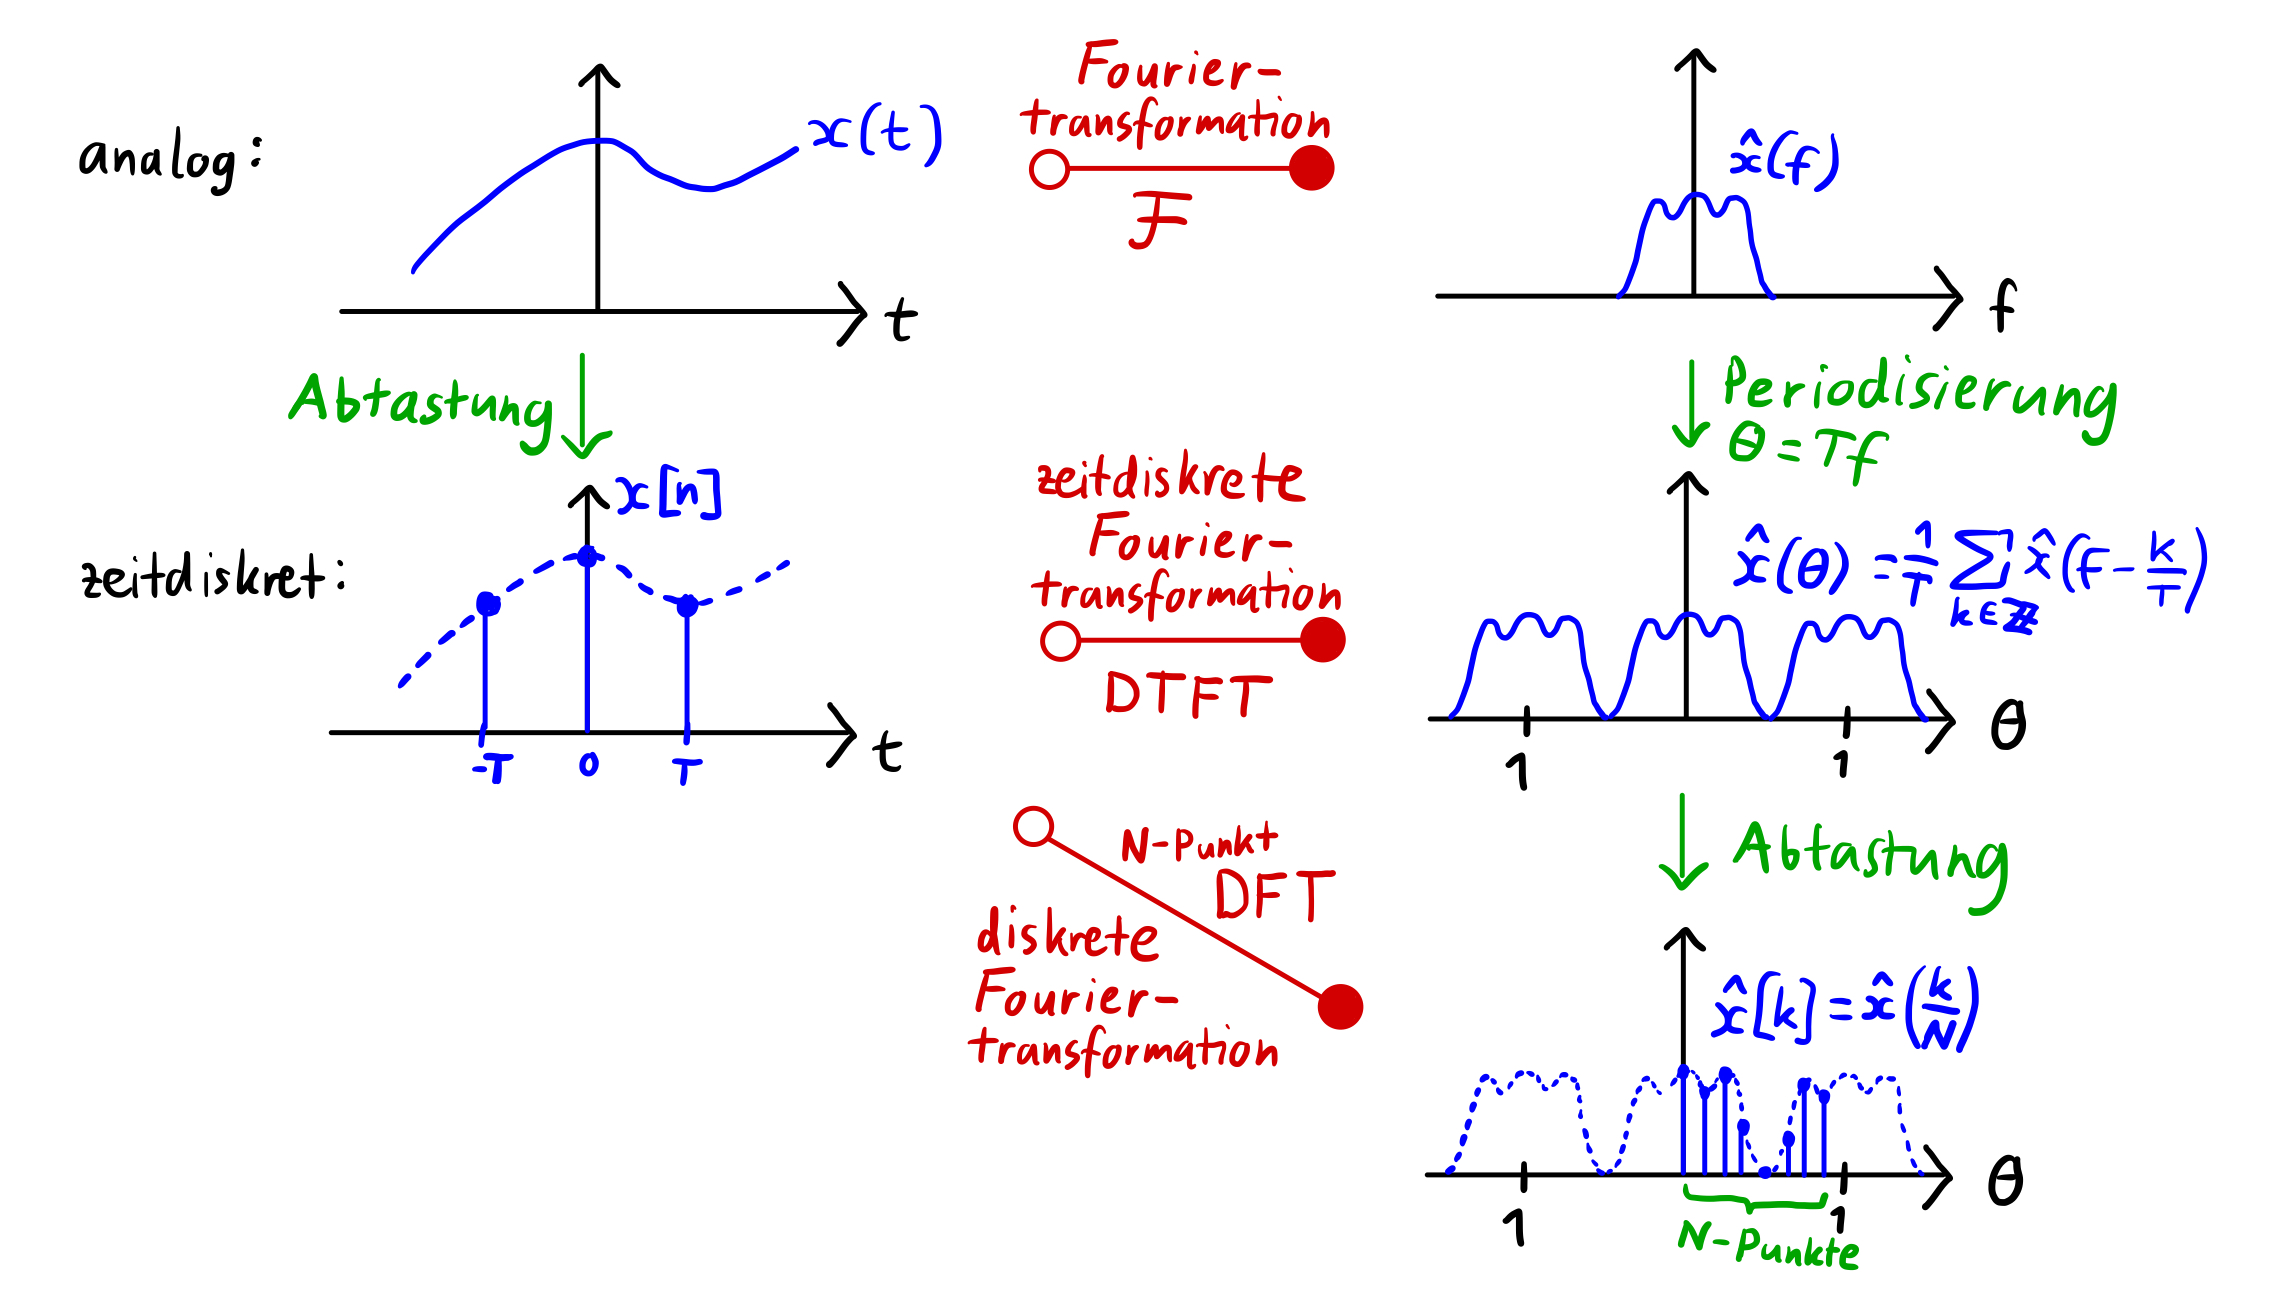
\includegraphics[width=0.8\linewidth]{docimgs/DFT_visuals.jpeg}
\end{center}

\vspace*{-0.5cm}
\subsection*{Matrixdarstellung}
\vspace*{-0.5cm}
Wir haben $\hat{x}[k] = \displaystyle\sum_{n=0}^{N-1} x[n]\omega_N^{kn}, \hspace{20pt} k \in \{ 0, \; 1, \; \dots, \; N-1 \}$ Somit:

$$\underbrace{\begin{bmatrix}
    \hat{x}[0] \\
    \hat{x}[1] \\
    \hat{x}[2] \\
    \vdots \\
    \hat{x}[N-1]
\end{bmatrix}}_{=: \hat{\mathbf{x}}} = \underbrace{\begin{bmatrix}
    1 & 1 & 1 & \cdots & 1 \\
    1 & \omega_N & \omega_N^2 & \cdots & \omega_N^{N-1} \\
    1 & \omega_N^2 & \omega_N^4 & \cdots & \omega_N^{2(N-1)} \\
    \vdots & \vdots & \vdots & \ddots & \vdots \\
    1 & \omega_N^{N-1} & \omega_N^{2(N-1)} & \cdots & \omega_N^{(N-1)^2}
\end{bmatrix}}_{\text{DFT-Matrix } F_N} \underbrace{\begin{bmatrix}
    x[0] \\
    x[1] \\
    x[2] \\
    \vdots \\
    x[N-1]
\end{bmatrix}}_{\mathbf{x}}$$


\fcolorbox{darkblue}{lightblue}{%
    \parbox{\dimexpr\linewidth-2\fboxsep-2\fboxrule\relax}{
        Somit erhalten wir: \\
        \noindent
        \begin{minipage}[t]{0.45\textwidth}
            \vspace*{0.1cm}
            \begin{itemize}
                \item[] \textbf{DFT}
                \item[] $\hat{\mathbf{x}} = F_N \mathbf{x}$
            \end{itemize}
            \vspace*{0.1cm}
        \end{minipage}%
        \hfill%
        \begin{minipage}[t]{0.45\textwidth}
            \vspace*{0.1cm}
            \begin{itemize}
                \item[] \textbf{IDFT}
                \item[] $\mathbf{x} = \frac{1}{N}F_N^H \hat{\mathbf{x}}$
            \end{itemize}
            \vspace*{0.1cm}
        \end{minipage}
    }%
}

Die Spalten von $F_N$ sind orthogonal aufeinander. Sei $\mathbf{f}_i$ die $i-$te Spalte von $F_N$. Es gilt $\langle \mathbf{f}_r, \; \mathbf{f}_s \rangle = \delta_{r,s}$

Es gilt $F_N F_N^H = N I_N$, wobei $I_N$ die Identitätsmatrix der Dimension $N$ ist.

\subsection*{Zyklische Faltung}
\vspace*{-0.5cm}
\fcolorbox{darkblue}{lightblue}{%
    \parbox{\dimexpr\linewidth-2\fboxsep-2\fboxrule\relax}{
    \vspace*{0.15cm}
    $$\vspace*{-0.5cm} x_3[l] = \sum_{n=0}^{N-1} x_1[n]x_2[l-n] = \sum_{n=0}^{N-1} x_1[l-n] x_2[n]$$
    $$\vspace*{-0.5cm}\verticaltransform{\text{DFT}}{1}{}{} \hspace{58pt}$$
    $$\hat{x}_3[k] = \hat{x}_1[k] \cdot \hat{x}_2[k]$$
}}%


\pagebreak

\subsection*{Diskrete Filter}


Wir haben gesehen, dass die DFT eines zeitdiskreten Signals der Länge $N$ einer Abtastung von $\hat{x}(\theta)$ entspricht, wobei die Abtastfrequenz $\frac{1}{N}$ ist.
$$\hat{x}[k] = \left.\hat{x}(\theta)\right|_{\theta = \frac{k}{N}}, \hspace{20pt} k = 0, \; 1, \; \dots, \; N-1$$

Das entspricht der \textcolor{red}{kritischen Abtastung} ($N \times N$ Matrix), aber was passiert bei Über-/Unterabtastung?

\subsection*{Überabtastung ($M > N$)}
\vspace*{-0.5cm}
$$\hat{x}\left(\frac{k}{M}\right) = \sum_{n=0}^{N-1}x[n]e^{-2 \pi i k \frac{n}{M}}, \hspace*{20pt} k = 0, \; 1, \; \dots, \; M-1$$
In Matrixform sieht das wie folgt aus:
$$\hat{\mathbf{x}} = \underbrace{\begin{bmatrix}
    1 & 1 & 1 & \cdots & 1 \\
    1 & \omega_M & \omega_M^2 & \cdots & \omega_M^{N-1} \\
    \vdots & \vdots & \vdots & \ddots & \vdots \\
    1 & \omega_M^{M-1} & \omega_M^{2(M-1)} & \cdots & \omega_M^{(N-1)(M-1)}
\end{bmatrix}}_{\text{Matrix }F_0} \mathbf{x} \hspace{20pt} \omega_M = e^{-\frac{2 \pi i}{M}}$$

\begin{itemize}
    \item $\mathbf{x} \in \mathbb{C}^{N \times 1}$ (Länge $N$) und $\hat{\mathbf{x}} \in \mathbb{C}^{M \times 1}$ (Länge $M$)
    \item $F_0 \in \mathbb{C}^{M\times N}$, ($M > N$) hat mehr Zeilen als Spalten
    \item Aus $\hat{\mathbf{x}}$ (DFT-Vektor) können wir mithilfe einer Pseudoinversen $\mathbf{x}$ zurückgewinnen.
    \item Für die Rücktransformation gilt: $\mathbf{x} = \displaystyle\frac{1}{M} F_0^H \hat{\mathbf{x}}$, was folgendem Ausdruck entspricht:
\end{itemize}
$$x[n] = \frac{1}{M} \sum_{k=0}^{M-1} \hat{x}[k]\omega_M^{-kn}, \hspace{20pt} n = 0, \; 1, \; \dots, \; N-1$$


\subsection*{Unterabtastung ($M < N$)}
\vspace*{-0.5cm}

\vfill \null
\pagebreak

\section*{Fast Fourier Transform (FFT)}
\vspace*{-0.5cm}
Die FFT ist ein Algorithmus, welcher die DFT effizient berechnet. Konkret braucht eine $N-$Punkt DFT $\mathcal{O}(N^2)$ Operationen. Für eine $N-$Punkt DFT mit $N=2^n, \; n \in \mathbb{N}$ kann der Rechenaufwand mittels FFT auf $4N \log_2(N)$, also auf $\mathcal{O}(N\log(N))$ reduziert werden.

\fcolorbox{darkblue}{lightblue}{%
    \parbox{\dimexpr\linewidth-2\fboxsep-2\fboxrule\relax}{
        \vspace*{0.1cm}
        \noindent
        \begin{minipage}[t]{0.45\textwidth}
            \vspace*{0.1cm}
            \begin{itemize}
                \item[] \textbf{DFT} ist in $\mathcal{O}(N^2)$
            \end{itemize}
            \vspace*{-0.1cm}
        \end{minipage}%
        \hfill%
        \begin{minipage}[t]{0.45\textwidth}
            \vspace*{0.1cm}
            \begin{itemize}
                \item[] \textbf{FFT} ist in $\mathcal{O}(N\log(N))$
            \end{itemize}
            \vspace*{-0.1cm}
        \end{minipage}
    }%
}

Die DFT ist gegeben durch 
$$\hat{x}[k] = \sum_{n=0}^{N-1} x[n]\omega_N^{kn}, \hspace{20pt} k=0, \; 1, \; \dots, \; N-1$$

\textbf{Idee}: Wir zerlegen die $N-$Punkt DFT in zwei $\frac{N}{2}-$Punkt DFTs (geraden und ungeraden Anteil) und führen diesen Schritt rekursiv so lange durch, bis wir nur noch $2-$Punkt DFTs haben. Dafür nehmen wir an, dass unser Signal Länge $N=2^n, \; n \in \mathbb{N}$ hat.

\textcolor{red}{figure Rekursionsbaum}

Am Ende haben wir nur noch $2-$Punkte DFTs:
$$F_2 = \begin{bmatrix}
    1 & 1 \\
    1 & \omega_2
\end{bmatrix} = \begin{bmatrix}
    1 & 1 \\
    1 & -1
\end{bmatrix} \implies \begin{array}{l}
    \hat{x}_r[0] = x_r[0] + x_r[1] \\
    \hat{x}_r[1] = x_r[0] - x_r[1]
\end{array}$$

\subsection*{FFT-Algorithmus von Cooley-Tukey}
\vspace*{-0.5cm}
Wir versuchen die $N-$Punkt DFT als zwei $\frac{N}{2}-$Punkt DFTs (geraden und ungeraden Anteil) zu schreiben. (Annahme: $N$ gerade, s.d. $\frac{N}{2} \in \mathbb{N}$ ist):

\begin{align*}
    \hat{x}[k] &= \sum_{n=0}^{N-1} x[n]\omega_N^{kn} = \sum_{n\text{ even}} x[n]\omega_N^{kn} + \sum_{n\text{ odd}} x[n]\omega_N^{kn} \\
    &= \sum_{l=0}^{\frac{N}{2}-1} x[2l]\omega_N^{k\cdot 2l} + \sum_{l=0}^{\frac{N}{2}-1} x[2l+1]\omega_N^{k(2l+1)} \\
    &= \sum_{l=0}^{\frac{N}{2}-1}x[2l]\left(\omega_N^2\right)^{kl} + \omega_N^k \sum_{l=0}^{\frac{N}{2}-1} x[2l+1] \left(\omega_N^2\right)^{kl}
\end{align*}

\textbf{Kunstgriff}: $\omega_N^2 = e^{-\frac{4 \pi i}{N}} = e^{-\frac{2 \pi i}{(N/2)}} = \omega_{\frac{N}{2}}$

\fcolorbox{darkblue}{lightblue}{%
    \parbox{\dimexpr\linewidth-2\fboxsep-2\fboxrule\relax}{
        \vspace*{0.1cm}
        $$\implies \underbrace{\sum_{l=0}^{\frac{N}{2}-1}x[2l]\omega_{\frac{N}{2}}^{kl}}_{=: \hat{g}[k]} + \omega_N^k \underbrace{\sum_{l=0}^{\frac{N}{2}-1} x[2l+1] \omega_{\frac{N}{2}}^{kl}}_{=: \hat{u}[k]}$$
    }%
}

Es folgt $\hat{x}[k] = \hat{g}[k] + \omega_N^k \hat{u}[k], \hspace{12pt} k = 0, \; 1, \; \dots, \; N-1$ wobei $\hat{g}[k]$ und $\hat{u}[k]$ $\frac{N}{2}-$Punkt DFTs sind, d.h.

$$\hat{g}[k] = \hat{g}\left[k + \frac{N}{2}\right] \hspace*{30pt} \hat{u}[k] = \hat{u}\left[k + \frac{N}{2}\right]$$


\vfill \null
\pagebreak


\begin{tikzpicture}
    % Define the box size and grid spacing
    \draw[step=0.5cm,gray!50,very thin] (0,0) grid (16.5,21
    ); % (0,0) is bottom-left corner, (10,10) is top-right corner
\end{tikzpicture}

\pagebreak

\section*{Prüfungsinformationen}
\vspace*{-0.5cm}
\begin{itemize}
    \item Die Prüfung dauert 180 min (3 Stunden).
    \item Es gibt 4 Aufgaben, die je 25 Punkte geben. (ca. 45 min pro Aufgabe)
    \item Einziges Hilfsmittel ist die Formelsammlung.
\end{itemize}

\subsection*{Kontur der Prüfung}
\vspace*{-0.5cm}
\begin{enumerate}
    \item Analoge Signale und Systeme, Systemeigenschaften
    \item Abtasttheorem (Mischung analoge und zeitdiskrete Signale)
    \item Zeitdiskrete Signale (entweder DTFT oder $\mathcal{Z}-$Transformation)
    \item DFT
\end{enumerate}

\subsection*{Tipps für die Prüfung}
\vspace*{-0.5cm}
\begin{itemize}
    \item Es gibt 20 alte Prüfungen. Löst möglichst viele davon, auch zweimal, wenn nötig!
    \item Die neueren Prüfungen sind relevanter und entsprechen in ihrer Kontur mehr derjenigen Prüfung, die ihr schreiben werdet.
    \item Nur 4 alte Prüfungen enthalten Aufgaben zu der $\mathcal{Z}-$Transformation. (Die letzten vier, das Thema ist also sehr prüfungsrelevant.) Schaut euch also die Aufgaben 114-122 dazu nochmals an.
    \item Schaut, dass ihr die Konzepte wie z.B. das Abtasttheorem gut versteht. Man kann in SST1 nämlich nicht einfach nur Aufgabentypen auswendig lernen, um die Prüfung zu bestehen.
    \item Substitutionen in Integralen und Summen müssen sitzen! Es werden zwar bei Rechenfehlern Teilpunkte gegeben, aber ihr verliert trotzdem einige  Punkte wollt ihr nicht vergeben.
    \item Vegesst nicht eure Lösungswege zu begründen, Achsenbeschriftungen bei Skizzen etc.
    \item Falls ihr Teilaufgaben nicht schafft, könnt ihr, wenn ihr übrige Zeit habt, trotzdem weiterrechnen (z.B. mit Parametern), vielleicht bekommt ihr dafür einige Punkte.
\end{itemize}

\end{document}